\documentclass[tikz, border=15pt]{standalone}
\usepackage{amsmath, amssymb}
\usetikzlibrary{arrows.meta, decorations.markings}

\begin{document}
	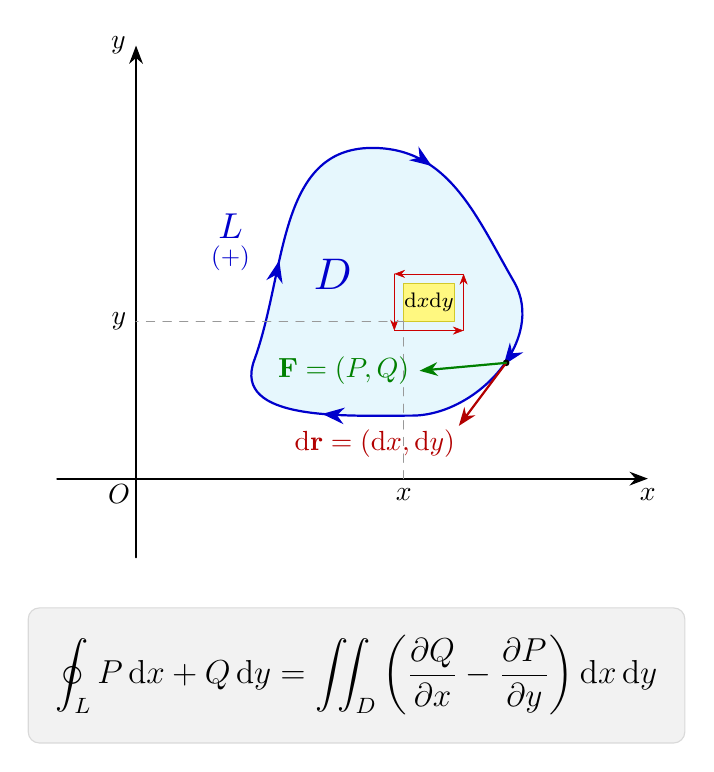
\begin{tikzpicture}[>=Stealth, line cap=round, line join=round]
		
		% ================= 1. 定义带有方向箭头的曲线样式 =================
		\tikzset{
			dir/.style={
				postaction={decorate, decoration={markings,
						mark=at position 0.12 with {\arrow[scale=1.2]{>}},
						mark=at position 0.38 with {\arrow[scale=1.2]{>}},
						mark=at position 0.65 with {\arrow[scale=1.2]{>}},
						mark=at position 0.88 with {\arrow[scale=1.2]{>}}
				}}
			}
		}
		
		% ================= 2. 绘制直角坐标系 =================
		\draw[->, thick] (-1, 0) -- (6.5, 0) node[below] {$x$};
		\draw[->, thick] (0, -1) -- (0, 5.5) node[left] {$y$};
		\node[below left, inner sep=2pt] at (0,0) {$O$};
		
		% ================= 3. 绘制闭合区域 D 与边界 L =================
		% 使用平滑的控制点绘制一个不规则闭合区域，逆时针方向为正
		\draw[thick, fill=cyan!10, dir, draw=blue!80!black]
		(1.5, 1.5) to[out=70, in=180] (3, 4.2)
		to[out=0, in=120] (4.8, 2.5)
		to[out=-60, in=0] (3.5, 0.8)
		to[out=180, in=-110] cycle;
		
		% 区域和边界标签
		\node[text=blue!80!black, scale=1.6] at (2.5, 2.6) {$D$};
		\node[text=blue!80!black, scale=1.3] at (1.2, 3.2) {$L$};
		\node[text=blue!80!black, scale=0.9] at (1.2, 2.8) {$(+)$}; % 表示正向
		
		% ================= 4. 绘制微观面积元与内部环流 (旋度物理直觉) =================
		\begin{scope}[shift={(3.4, 2.0)}, scale=0.8]
			% 面积微元
			\draw[fill=yellow!50, draw=yellow!80!black, thin] (0,0) rectangle (0.8, 0.6);
			\node[scale=0.95] at (0.4, 0.3) { {\footnotesize $\mathrm{d}x\mathrm{d}y$}};
			
			% 微观涡旋 (内部小环流相互抵消的示意)
			\draw[->, very thin, red!80!black] (-0.15, -0.15) -- (0.95, -0.15);
			\draw[->, very thin, red!80!black] (0.95, -0.15) -- (0.95, 0.75);
			\draw[->, very thin, red!80!black] (0.95, 0.75) -- (-0.15, 0.75);
			\draw[->, very thin, red!80!black] (-0.15, 0.75) -- (-0.15, -0.15);
		\end{scope}
		
		% 辅助线：标示内部微元的无穷小特性
		\draw[dashed, gray!80, thin] (3.4, 2.0) -- (3.4, 0) node[below, text=black] {$x$};
		\draw[dashed, gray!80, thin] (3.4, 2.0) -- (0, 2.0) node[left, text=black] {$y$};
		
		% ================= 5. 绘制边界上的矢量场与线元 =================
		\coordinate (P) at (4.7, 1.47); % 边界 L 上的某一点
		\fill[black] (P) circle (1.2pt);
		
		% 线微元 dr (相切于曲线)
		\draw[->, thick, red!70!black] (P) -- ++(-0.6, -0.8) node[below left, inner sep=1pt] {$\mathrm{d}\mathbf{r} = (\mathrm{d}x, \mathrm{d}y)$};
		
		% 矢量场 F
		\draw[->, thick, green!50!black] (P) -- ++(-1.1, -0.1) node[left] {$\mathbf{F} = (P, Q)$};
		
		% ================= 6. 底部公式框 (格林公式) =================
		\node[fill=gray!10, rounded corners, inner sep=10pt, draw=gray!30] at (2.8, -2.5) {
			\large $\displaystyle\oint_{L} P\,\mathrm{d}x + Q\,\mathrm{d}y = \iint_{D} \left( \frac{\partial Q}{\partial x} - \frac{\partial P}{\partial y} \right) \mathrm{d}x\,\mathrm{d}y$
		};
		
	\end{tikzpicture}
\end{document}